% Lecture Template for ME3023 -  Measurements in Mechanical Systems - Tennessee Technological University
% Spring 2020 - Summer 2020 - Fall 2020 - Spring 2021 - Summer 2021 - Fall 2023
% Tristan Hill, May 07, 2020 - June 12, 2020 - July 08, 2020 - Novemeber 02, 2020 - March 28, 2021 - May 25, 2021 - August 21, 2022 - September 02, 2023 - September 09, 2023

% Fall 2023 - condensing and streamlining lectures by combining topics into a single PDF under the module name
%			  this will simplify file and link management as well as make lectures easier to use in class
%			- added image/ to clean directory and reduce redundancy, specific to module for now  

% Module Name: - Steady State Circuits
% Topic 1 - Components, Units, and Symbols
% Topic 2 - Fundamental Laws
% Topic 3 - Circuit Applications


\documentclass[fleqn]{beamer} % for presentation (has nav buttons at bottom)

\usepackage{../measurements_lectures}

\author{ME3023 - Measurements in Mechanical Systems} % original formatting from Mike Renfro, September 21, 2004

\newcommand{\MNUM}{4\hspace{2mm}} % module number 
\newcommand{\moduletitle}{Electrical Signals}

\newcommand{\sectionItitle}{Classification of Signals}
\newcommand{\sectionIItitle}{Signal Analysis}
\newcommand{\sectionIIItitle}{Sampling and Aliasing}

\newcommand{\sectionIsubsectionItitle}{Introduction to Signal Concepts}
\newcommand{\sectionIsubsectionIItitle}{Analog, Discrete, or Digital}
\newcommand{\sectionIsubsectionIIItitle}{Static or Dynamic}
\newcommand{\sectionIsubsectionIVtitle}{Deterministic or Non-Deterministic}

\newcommand{\sectionIIsubsectionItitle}{Signal Mean Value}
\newcommand{\sectionIIsubsectionIItitle}{Power Dissipation}
\newcommand{\sectionIIsubsectionIIItitle}{Signal Root Mean Square (RMS) Value}
\newcommand{\sectionIIsubsectionIVtitle}{Discrete-Time or Digital Signals}

\newcommand{\sectionIIIsubsectionItitle}{Sampling}
\newcommand{\sectionIIIsubsectionIItitle}{The Aliasing Phenomenon}
\newcommand{\sectionIIIsubsectionIIItitle}{Example by Hand}
\newcommand{\sectionIIIsubsectionIVtitle}{MATLAB Example}

\newcommand{\btVFill}{\vskip0pt plus 1filll}

\newcommand{\uhspc}{\underline{\hspace{20 mm}}}


% custom box
\newsavebox{\mybox}

\title{Lecture Module - \moduletitle}

\date{Mechanical Engineering\vspc Tennessee Technological University}

\begin{document}

	\lstset{language=MATLAB,basicstyle=\ttfamily\small,showstringspaces=false}

	\frame{\titlepage \center\begin{framed}\Large \textbf{Module \MNUM - \moduletitle}\end{framed} \vspace{5mm}}

	% Module Outline
	\begin{frame} 
		\large \textbf{Module \MNUM - \moduletitle} \vspace{3mm}\\

		\begin{itemize}
			\item Topic 1 - \hyperlink{sectionI}{\sectionItitle} \vspc % section I
			\item Topic 2 - \hyperlink{sectionII}{\sectionIItitle} \vspc % section II
			\item Topic 3 - \hyperlink{sectionIII}{\sectionIIItitle} \vspc % section III
		\end{itemize}

	\end{frame}

	% section I
	\section{\sectionItitle}\label{sectionI}

		% section I Outline
		\begin{frame} 
			\large \textbf{Topic 1 - \sectionItitle} \vspace{3mm}\\

			\begin{itemize}
				\item \hyperlink{sectionIsubsectionI}{\sectionIsubsectionItitle} \vspc %  section I subsection I
				\item \hyperlink{sectionIsubsectionII}{\sectionIsubsectionIItitle} \vspc % section I subsection II
				\item \hyperlink{sectionIsubsectionIII}{\sectionIsubsectionIIItitle} \vspc % section I subsection III
				\item \hyperlink{sectionIsubsectionIV}{\sectionIsubsectionIVtitle} \vspc % section I subsection IV
			\end{itemize}
		\end{frame}
		
		% section I subsection I 
		\subsection{\sectionIsubsectionItitle}\label{sectionIsubsectionI}

			\begin{frame}
				\frametitle{\sectionIsubsectionItitle}
				
		\begin{multicols}{2}
		{\PR Signal}, {\RD Amplitude}, and {\BL Frequency}\vspace{2mm}\\
		\includegraphics[scale=.3]{images/amplitude_frequency.png} 
		%\includegraphics[scale=.25]{unit_circle.png}
		
		%\vspace*{10mm}
		
		{\it The shape and form of a {\PR \uhspc } are often referred to as its {\PN \uhspc}.
		The {\PN \uhspc} contains information about the magnitude and {\RD \uhspc}, which indicate the size of
		the input quantity, and the {\BL \uhspc}, which indicates the way the {\PR \uhspc} changes in time. }\vspace{5mm}\\
		
		\end{multicols}
		%\btVFill
		\tiny{Text: Theory and Design for Mechanical Measurements}	



			\end{frame}

			\begin{frame}
				\frametitle{\sectionIsubsectionItitle}

						\bigskip
		
		{\it A {\PR \uhspc} is the physical information about a measured variable being transmitted
		between a process and the measurement system, between the stages of a measurement system, or as
		the output from a measurement system. } \\
	
		\includegraphics[scale=.07]{images/computer_motherboard.jpg} 
		\includegraphics[scale=.06]{images/curiosity_on_mars.jpg} 
		\includegraphics[scale=.22]{images/tesla_underhood.jpg}
		
		\btVFill
		\tiny{Images: Wikipedia}	

		

			\end{frame}

		% section I subsection II
		\subsection{\sectionIsubsectionIItitle}\label{sectionIsubsectionII}

			\begin{frame}
				\frametitle{\sectionIsubsectionIItitle}

					    \begin{itemize}
			\item \textbf{\uhspc Signal- magnitude is continuous in time }  \vspace{3mm} \\
			\item \textbf{\uhspc Signal- magnitude at points in time}  \vspace{3mm} \\
			\textbf{ \hspace*{15mm} - sampling at repeated time intervals}  \vspace{3mm} \\
			\item \textbf{\uhspc Signal- exists in discrete points in time}  \vspace{3mm} \\
			\textbf{ \hspace*{15mm} - magnitude is also discrete}  \vspace{3mm} \\
		\end{itemize}



			\end{frame}

			\begin{frame}
				\frametitle{\sectionIsubsectionIItitle}


		{\it {\RD Analog} describes a signal that is
		continuous in time. Because physical variables tend to be continuous, an analog signal provides a
		ready representation of their time-dependent behavior. }

		\vspace{30mm}
		Examples: voltage in a circuit
%	\includegraphics[scale=.25]{topic2_histogram_fig1}
		\btVFill
		\tiny{Text: Theory and Design for Mechanical Measurements}	
				


			\end{frame}


			\begin{frame}

						\bigskip  
			
		{\it ...a {\GR discrete time} signal, for which information about the
		magnitude of the signal is available only at discrete points in time. A discrete time signal usually
		results from the sampling of a continuous variable at repeated finite time intervals. }

%	\includegraphics[scale=.25]{topic2_histogram_fig2}
		\vspace{30mm}
		Examples:
		\btVFill
		\tiny{Text: Theory and Design for Mechanical Measurements}	

			\end{frame}

			\begin{frame}
			\bigskip 
			{\it A {\BL digital} signal has two important characteristics. First, a digital signal
			exists at discrete values in time, like a discrete time signal. Second, the magnitude of a digital signal
			is discrete, determined by a process known as {\PR quantization} at each discrete point in time. }

%	\includegraphics[scale=.25]{topic2_histogram_fig3}
		\vspace{30mm}
		Examples:
		\btVFill
		\tiny{Text: Theory and Design for Mechanical Measurements}	
			\end{frame}





		% section I subsection III
		\subsection{\sectionIsubsectionIIItitle}\label{sectionIsubsectionIII}
			\begin{frame} 
				\frametitle{\sectionIsubsectionIIItitle}

				\bigskip

Signals may be characterized as either static or
dynamic. A static signal does not vary with time.

A dynamic signal is defined as a time-dependent signal. In general, dynamic signal waveforms,
y(t), may be classified as shown in Table 2.1.
	
\btVFill
\tiny{Text: Theory and Design for Mechanical Measurements}	



			\end{frame}	

			\begin{frame} 
				\frametitle{\sectionIsubsectionIIItitle}

				
			\end{frame}	

		% section I subsection IV
		\subsection{\sectionIsubsectionIVtitle}\label{sectionIsubsectionIV}	

			\begin{frame}
				\frametitle{\sectionIsubsectionIVtitle}

				\bigskip

A deterministic signal varies in time in a predictable
manner, such as a sine wave, a step function, or a ramp function, as shown in Figure 2.5. A signal is
steady periodic if the variation of the magnitude of the signal repeats at regular intervals in time.

Also described in Figure 2.5 is a non-deterministic signal that has no discernible pattern of
repetition. A non-deterministic signal cannot be prescribed before it occurs, although certain characteristics of the signal may be known in advance.

\btVFill
\tiny{Text: Theory and Design for Mechanical Measurements}
		
				
			\end{frame}

			\begin{frame}
				\frametitle{\sectionIsubsectionIVtitle}

\bigskip

\includegraphics[scale=.15]{images/table_2_1.png}

\btVFill
\tiny{Table 2.1 : Theory and Design for Mechanical Measurements}
				
		

			\end{frame}

	
	% Section II
	\section{\sectionIItitle}\label{sectionII}

		% section II Outline
		\begin{frame}
			\large \textbf{Topic 2 - \sectionIItitle} \vspace{3mm}\\

			\begin{itemize}
				\item \hyperlink{sectionIIsubsectionI}{\sectionIIsubsectionItitle} \vspc %  section II subsection I
				\item \hyperlink{sectionIIsubsectionII}{\sectionIIsubsectionIItitle} \vspc % section II subsection II
				\item \hyperlink{sectionIIsubsectionIII}{\sectionIIsubsectionIIItitle} \vspc % section II subsection III
				\item \hyperlink{sectionIIsubsectionIV}{\sectionIIsubsectionIVtitle} \vspc % section II subsection IV
			\end{itemize}

		\end{frame}

		% section II subsection I
		\subsection{\sectionIIsubsectionItitle}\label{sectionIIsubsectionI}

			\begin{frame}[label=sectionIIsubsectionI]
				\frametitle{\sectionIIsubsectionItitle}

						\begin{multicols}{2}
		\includegraphics[scale=.30]{images/amplitude_frequency.png} 
		
 Mean Value \[\bar{y}\equiv \frac{\int\limits_{t_1}^{t_2} y(t)dt}{\int\limits_{t_1}^{t_2} dt} \]
		\end{multicols}
		\btVFill
		\tiny{Text: Theory and Design for Mechanical Measurements}

		
			\end{frame}

		    \begin{frame}[label=sectionIIsubsectionI]
				\frametitle{\sectionIIsubsectionItitle}

				Dissipation - Time Rate of Energy Dissipation    \[ P=I^2R \]  
	
	Total Electrical Energy \hspace{5mm} \[ E =\int\limits_{t_1}^{t_2}P dt=\int\limits_{t_1}^{t_2}[I(t)]^2R dt \]
		
		



			\end{frame}	

		% section II subsection II
		\subsection{\sectionIIsubsectionIItitle}\label{sectionIIsubsectionII}

			\begin{frame}
				\frametitle{\sectionIIsubsectionIItitle}


	\begin{itemize}
	\item For a cyclically alternating electric current, RMS is equal to the value of the direct current that would produce the same average power dissipation in a resistive load.
	\item In Estimation theory, the root mean square error of an estimator is a measure of the imperfection of the fit of the estimator to the data.  
	\item The RMS value of a signal having a zero mean is a statistical measure of the magnitude of the fluctuations in the signal.
	\end{itemize}


			\end{frame}

		% section II subsection III
		\subsection{\sectionIIsubsectionIIItitle}\label{sectionIIsubsectionIII}

			\begin{frame}
				\frametitle{\sectionIIsubsectionIIItitle}

				\bigskip

\[(I_e)^2R(t_2-t_1)=\int\limits_{t_1}^{t_2}[I(t)]^2R dt\]

\[I_e = \sqrt{\frac{1}{t_2-t_1}\int\limits_{t_1}^{t_2}[I(t)]^2 dt} \]

\vspace{10mm}

\[y_{rms} = \sqrt{\frac{1}{t_2-t_1}\int\limits_{t_1}^{t_2}[y]^2 dt} \]


\btVFill
\tiny{Table 2.1 : Theory and Design for Mechanical Measurements}


			\end{frame}

			\begin{frame}
				\frametitle{\sectionIIsubsectionIIItitle}

\bigskip

\[\bar{y}=\frac{1}{N}\sum\limits_{i=0}^{N-1} y_i\] \vspace{10mm}\\	
\[y_{RMS}=\sqrt{\frac{1}{N}\sum\limits_{i=0}^{N-1} y_i^2}\] \vspace{10mm}\\	

\btVFill
\tiny{Text: Theory and Design for Mechanical Measurements}	
			

			\end{frame}

			\begin{frame}
			\frametitle{\sectionIIsubsectionIIItitle}




\btVFill
\tiny{Table 2.1 : Theory and Design for Mechanical Measurements}	



			\end{frame}

		% section II subsection IV 
		\subsection{\sectionIIsubsectionIVtitle}\label{sectionIIsubsectionIV}

			\begin{frame}
				\frametitle{\sectionIIsubsectionIVtitle}


			\end{frame}

			\begin{frame}
				\frametitle{\sectionIIsubsectionIVtitle}


			\end{frame}
		
	
	% Section III
	\section{\sectionIIItitle}\label{sectionIII}

		% section III Outline
		\begin{frame}
			\large \textbf{Topic 3 - \sectionIIItitle} \vspace{3mm}\\

			\begin{itemize}
				\item \hyperlink{sectionIIIsubsectionI}{\sectionIIIsubsectionItitle} \vspc %  section III subsection I
				\item \hyperlink{sectionIIIsubsectionII}{\sectionIIIsubsectionIItitle} \vspc % section III subsection II
				\item \hyperlink{sectionIIIsubsectionIII}{\sectionIIIsubsectionIIItitle} \vspc % section III subsection III
				\item \hyperlink{sectionIIIsubsectionIV}{\sectionIIIsubsectionIVtitle} \vspc % section III subsection IV
			\end{itemize}

		\end{frame}

		% section III subsection I
		\subsection{\sectionIIIsubsectionItitle}\label{sectionIIIsubsectionI}

			\begin{frame}
				\frametitle{\sectionIIIsubsectionItitle}
				\bigskip
						...
						A discrete time signal usually
						results from the sampling of a continuous variable at repeated finite time intervals.
						...	
						\includegraphics[scale=.3]{images/sampling_fig7_1.png}
					
						\btVFill
						\tiny{Text,Figure: Theory and Design for Mechanical Measurements Ch. 7}
			
			\end{frame}

		% section III subsection II
		\subsection{\sectionIIIsubsectionIItitle}\label{sectionIIIsubsectionII}	

			\begin{frame}
				\frametitle{\sectionIIIsubsectionIItitle}
				\bigskip
				\includegraphics[scale=.2]{images/aliasing_fig7_2.png}


				\btVFill
				\tiny{Figure: Theory and Design for Mechanical Measurements Ch. 7}	
					
			\end{frame}

		% section III subsection III
		\subsection{\sectionIIIsubsectionIItitle}\label{sectionIIIsubsectionIII}

			\begin{frame}
				\frametitle{\sectionIIIsubsectionIIItitle}
				\bigskip
				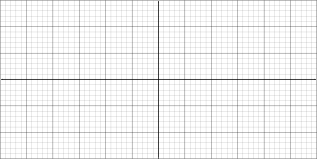
\includegraphics[scale=.35]{images/cartesian_6x12.png}


				\btVFill
				\tiny{Image: T.Hill}		
		
			\end{frame}

			\begin{frame}
				\frametitle{\sectionIIIsubsectionIIItitle}



			\end{frame}

		% section III subsection IV
		\subsection{\sectionIIIsubsectionIVtitle}\label{sectionIIIsubsectionIV}	

			\begin{frame}
				\frametitle{\sectionIIIsubsectionIVtitle}
				\bigskip

				{\textbf Activity: Sampling Demonstration}

				Use the MATLAB program provided to accomplish the following:

				\begin{enumerate} \tiny

					\item Plot a sinusoidal signal $y(t)=Asin(\omega\cdot t)=Asin(2\pi f \cdot t)$ with an amplitude $A=10$ (units) and frequency $f=1000$ (Hz). This is the {\it ideal signal} source. 
					\begin{itemize} \tiny
						\item Include axis labels and gridlines. 
						\item Choose ampitude and time scales so that 15 to 20 periods or the waveform are shown. \vspace{5mm}\\
					\end{itemize} 
					\item Simulate the samping of the signal by plotting the same function with a reduced time step. Plot the sampled signal on the same figure. Use a different marker and include a legend to differentiate the signals. \vspace{5mm}\\ 

					\item Use your code to determine the minimum sampling frequency required to measure the following quantities (note: use the sampled signal only, the {\it ideal signal} is not accessible).	

					\begin{itemize} \tiny
						\item {\bf Frequency} of the {\it ideal signal}
						\item {\bf Amplitude} of the {\it ideal signal}
					\end{itemize}



				\end{enumerate}

				\btVFill

				\tiny
				{\textbf Deliverables: Submit answers to all questsions to the appropriate ilearn folder. If you work with a partner, include all names with the responses. All group members must submit the assignment.}
			
			\end{frame}

			\begin{frame}
				\frametitle{\sectionIIIsubsectionIVtitle}
				


			\end{frame}

\end{document}





